\subsubsection{Topología y niveles}

    La topología del modelo es una parte fundamental del estándar. RailTopoModel incluye el "principio de agregación", por el cual los elementos pueden ser agrupados en entidades mas grandes. En la Figura \ref{fig:RTM_1} se puede visualizar la estructura de capas propuesto por RailTopoModel.

    \begin{figure}[!h]
        \centering
        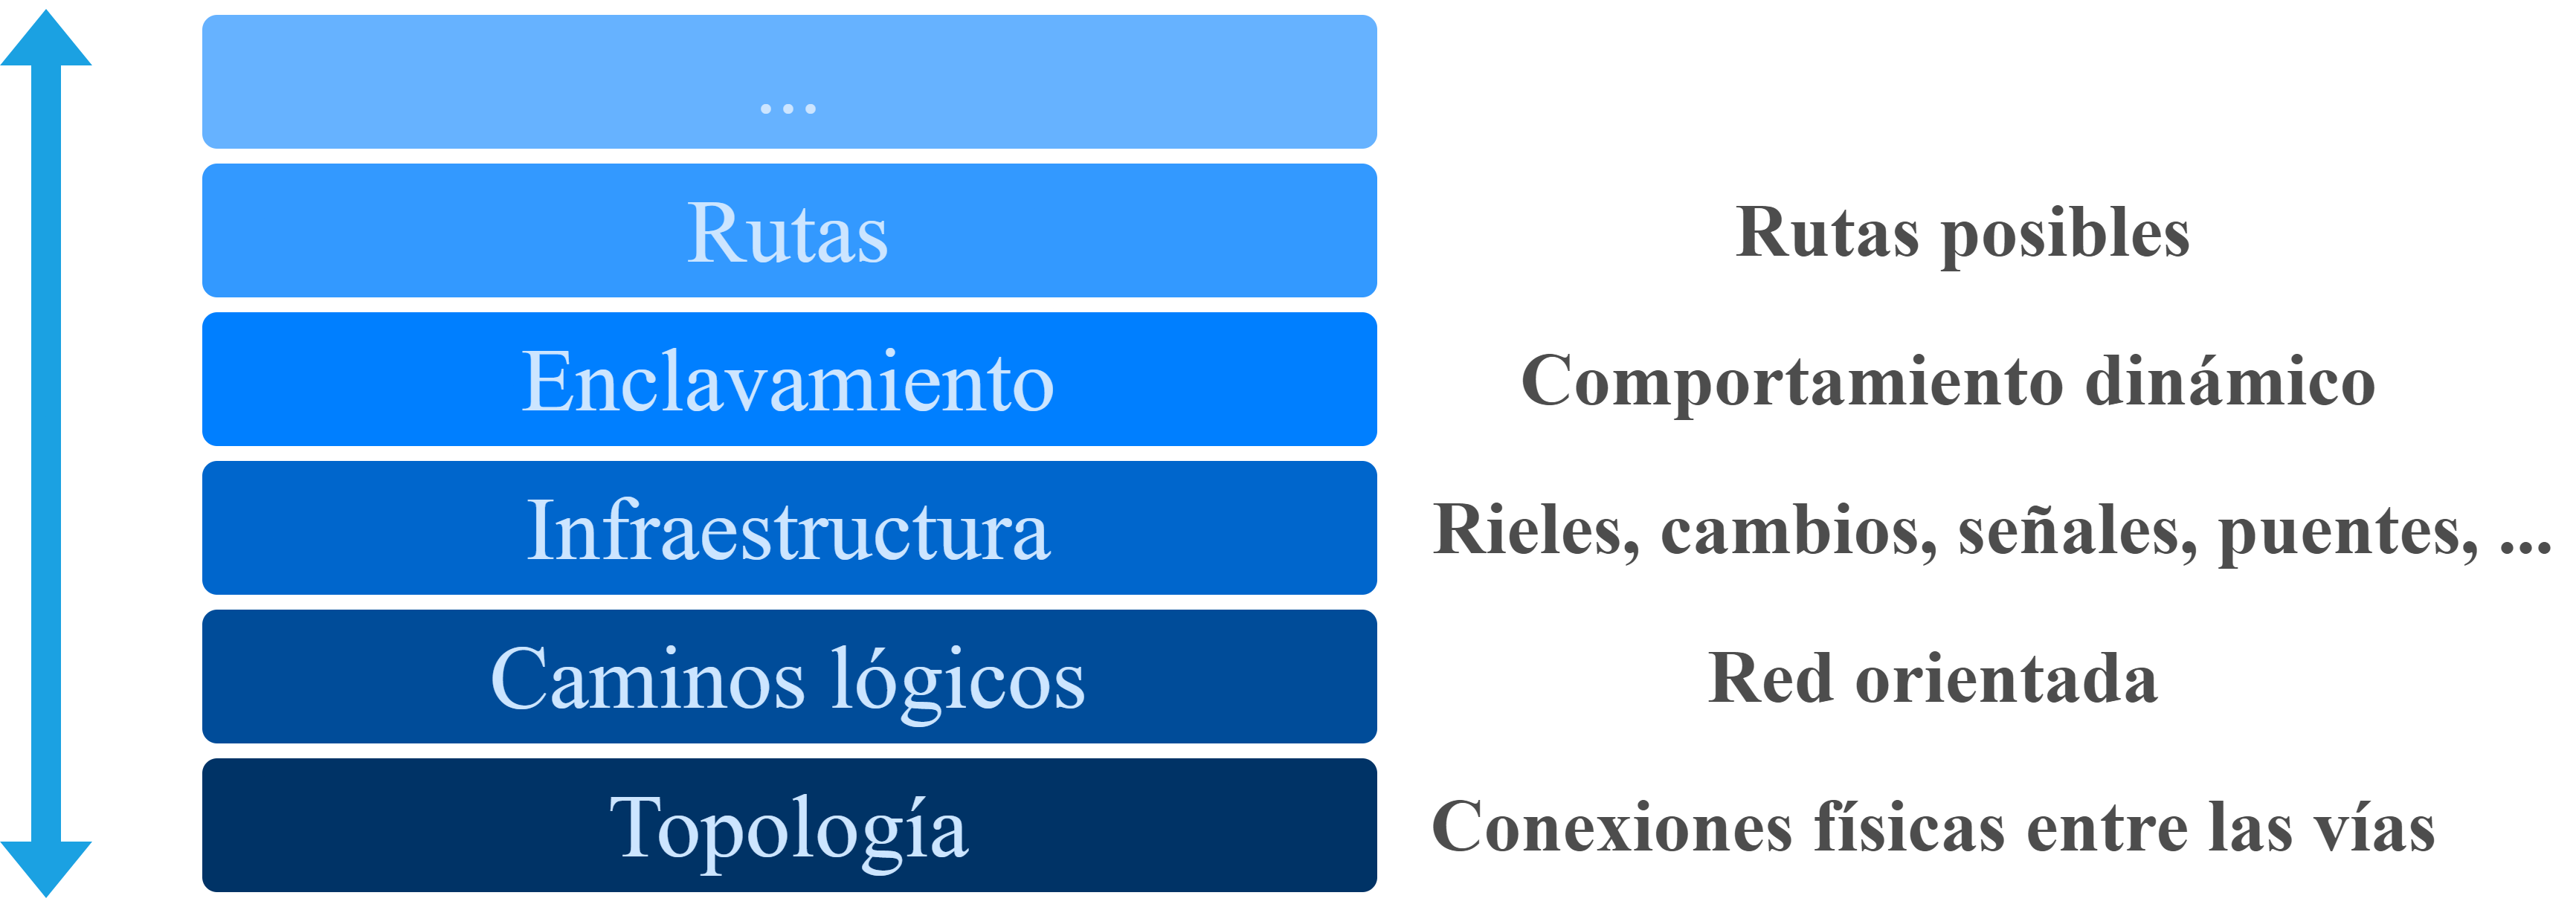
\includegraphics[width=1\textwidth]{Figuras/capas}
        \centering\caption{Estructura de capas de RailTopoModel.}
        \label{fig:RTM_1}
    \end{figure}
    
    La topología de la red está compuesta por los nodos (netElements) y las aristas (netRelations) que los conectan entre sí, lo cual constituye el nivel microscópico de la red. Cada nodo representa un tramo de vías que puede tener ciertos elementos ferroviarios asociados o ninguno. A su vez, los nodos pueden ser agrupados en diversos caminos lógicos, que son el conjunto de nodos cuyas relaciones y navegabilidad les permite constituir un camino físico entre ellos.

    A medida que se agrupan mas y mas cambios de vías junto con las plataformas y máquinas de cambios se constituye un punto de operación. La descripción en base a puntos de operación es a nivel mesoscópico, como se muestra en la Figura \ref{fig:RTM_2}, y es utilizado en logística. Las secciones de vía que no incluyen plataformas en las cuales las formaciones puedan detenerse se denominan secciones de líneas, o simplemente "líneas" dentro del modelo de RailTopoModel. La descripción que incluye tanto los puntos de operación como las secciones de líneas es a nivel macroscópico. Esta simplificación de la red es de gran importancia, ya que es ampliamente utilizada en los mapas ferroviarios de todas las estaciones del mundo: los puntos de operación son las estaciones y las secciones de línea son las vías que las comunican. 
    
    \begin{figure}[!h]
        \centering
        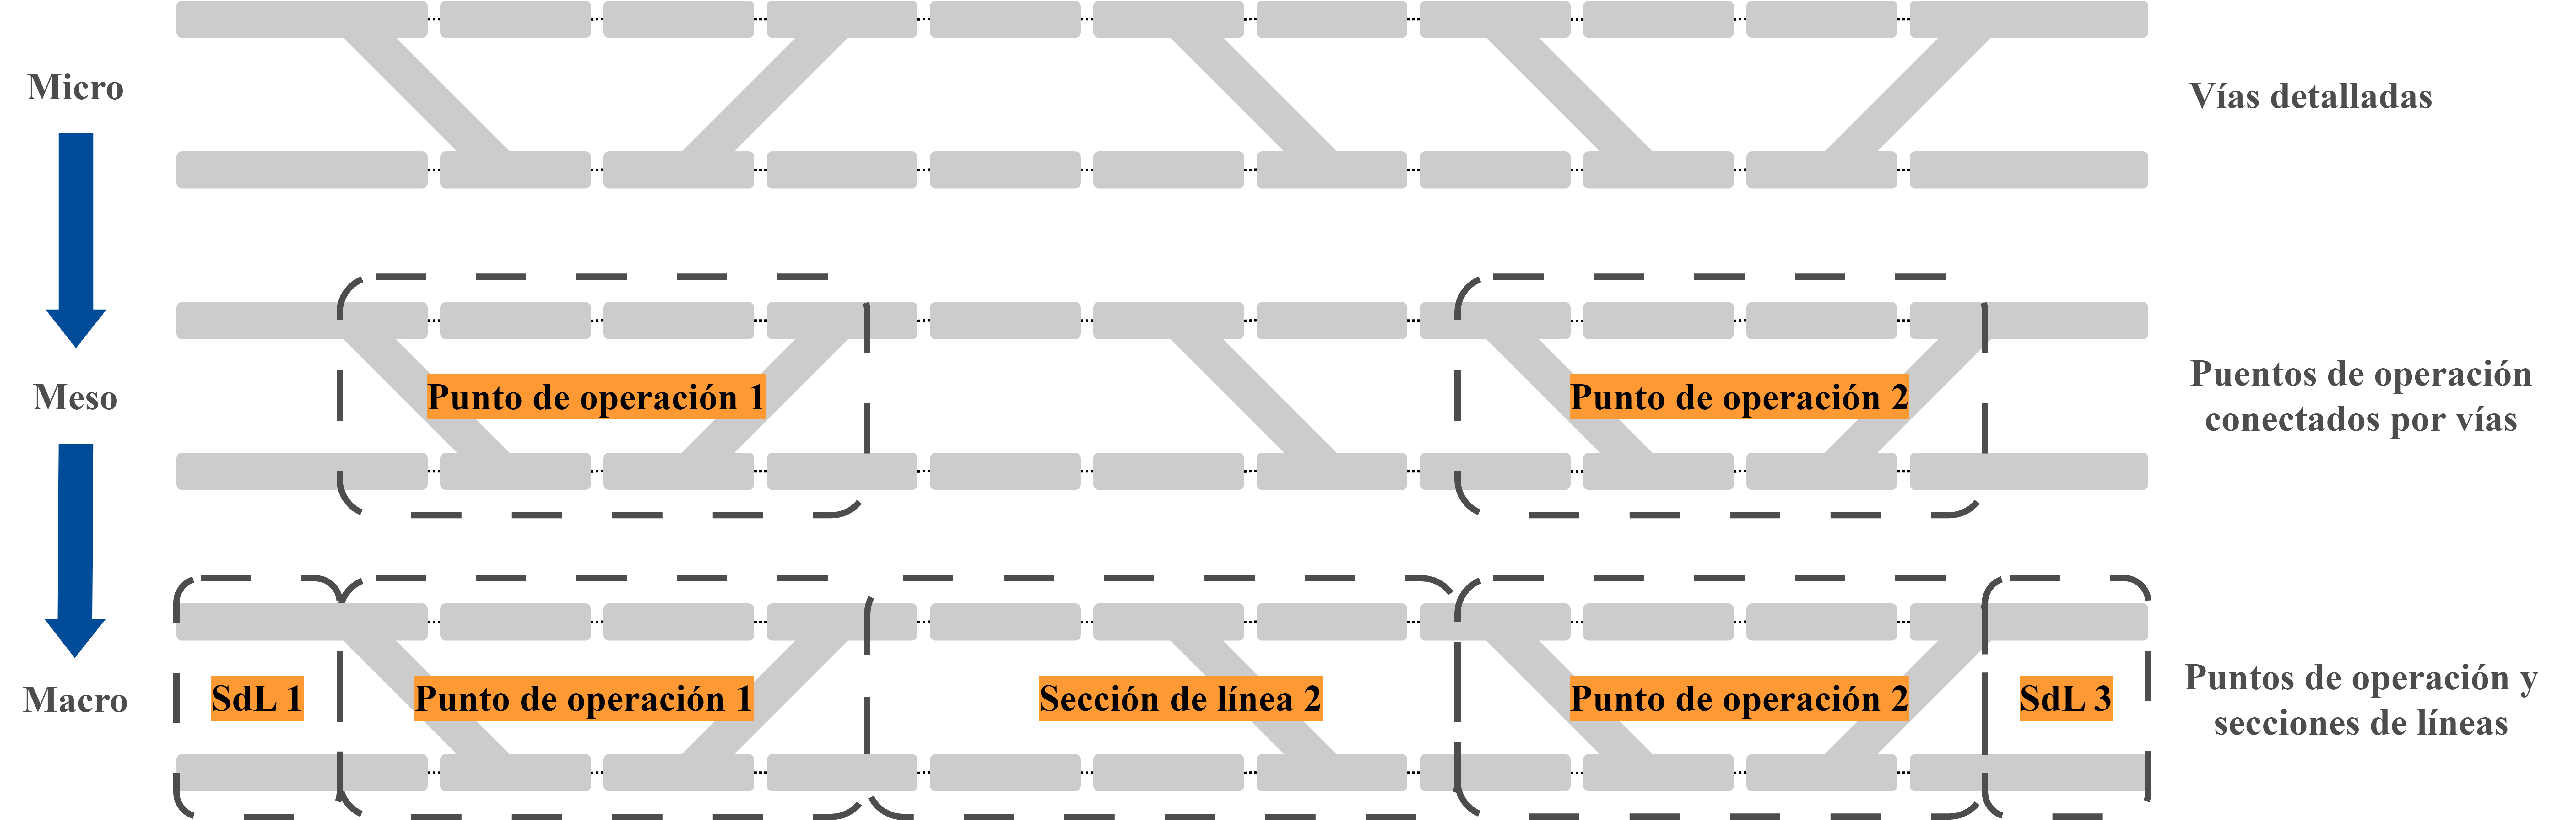
\includegraphics[width=1\textwidth]{Figuras/railtopomodel}
        \centering\caption{Niveles microscópico, mesoscópico y macroscópico.}
        \label{fig:RTM_2}
    \end{figure}
    
    Las instalaciones y sus propiedades constituyen todos los elementos ferroviarios asociados a un nodo. Estos representan elementos físicos del mundo real, pueden ser estáticos o dinámicos. Los elementos estáticos como los puentes, curvas y estaciones no alteran sus propiedades en ningún momento. Los elementos dinámicos como los pasos a nivel, máquinas de cambios o señales tienen algunas propiedades fijas, como la posición física del elemento, pero otras variables, como la posición mecánica de alguna de sus piezas o el estado eléctrico de sus circuitos.

    Un sistema de enclavamiento relaciona todos los módulos previamente mencionados. El sistema de enclavamientos modificará el estado de los elementos dinámicos, basados en el estado actual de los mismos, sometido a las restricciones impuestas por los elementos estáticos, buscando habilitar los caminos lógicos mas cortos y seguros entre un punto A y B.

    Finalmente, las rutas permitidas se obtienen a partir del estado de los elementos dinámicos decidido por el sistema y de definir el camino óptimo entre A y B que no comprometa la infraestructura del sistema. Todas las restricciones impuestas por las capas inferiores (caminos lógicos posibles, limitaciones de la infraestructura o estados previos que sean incompatibles con lo pedido) terminan emergiendo como un conjunto de rutas posibles de ser utilizadas, en detrimento de otras que, en ese instante de tiempo, no podrán ser habilitadas hasta que el estado del sistema se modifique.

    Como se puede apreciar, en este modelo, las rutas son una consecuencia de la infraestructura que se tiene y de los estados anteriores del sistema, producto de las rutas previamente pedidas. Un análisis completo de la topología e infraestructura permitiría obtener todo el conjunto de rutas posibles, para cualquier estado alcanzable por el sistema.